\documentclass[12pt]{article}
\usepackage{amsfonts, amssymb, amsmath, amsthm}
\usepackage[margin=1in]{geometry}
\usepackage{tikz}

\title{Explainer: Bonus Problem 2 (Rudin 7.21) --- Isometric Embedding into $\mathscr{C}(X)$}
\author{}
\date{}

\begin{document}
\maketitle

\section*{What's going on?}
Given \emph{any} metric space $(X, d)$, we embed it isometrically into the Banach space $\mathscr{C}(X)$ of bounded continuous functions on $X$ (with the sup norm). Then taking the closure gives a \textbf{completion} of $X$.

This is a very general and elegant construction: every metric space lives inside a complete one.

\section*{The embedding}

Fix a base point $a \in X$. For each $p \in X$, define $f_p : X \to \mathbb{R}$ by:
$$
f_p(x) = d(x,p) - d(x,a).
$$

\begin{center}
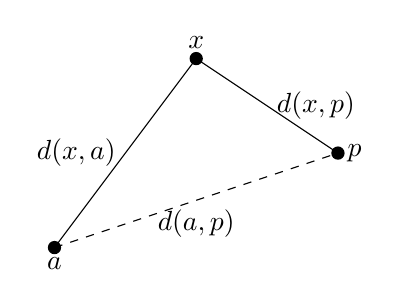
\begin{tikzpicture}[>=stealth, scale=1.2]
    \fill (0,0) circle (2pt) node[below] {$a$};
    \fill (3,1) circle (2pt) node[right] {$p$};
    \fill (1.5, 2) circle (2pt) node[above] {$x$};

    \draw (1.5,2) -- (3,1) node[midway, right] {$d(x,p)$};
    \draw (1.5,2) -- (0,0) node[midway, left] {$d(x,a)$};
    \draw[dashed] (0,0) -- (3,1) node[midway, below] {$d(a,p)$};
\end{tikzpicture}
\end{center}

$f_p(x)$ measures ``how much closer is $x$ to $a$ than to $p$?'' Subtracting $d(x,a)$ centers things so that $f_p(a) = 0 - 0 = 0$ always... wait, $f_p(a) = d(a,p) - d(a,a) = d(a,p)$. The subtraction of $d(x,a)$ ensures $f_p$ is bounded.

\section*{Step 1: $|f_p(x)| \leq d(a,p)$}

By the triangle inequality:
$$
d(x,p) - d(x,a) \leq d(a,p) \qquad \text{and} \qquad d(x,a) - d(x,p) \leq d(a,p).
$$
Both come from $d(x,p) \leq d(x,a) + d(a,p)$ (and the symmetric version). So $|f_p(x)| \leq d(a,p)$ for all $x$.

Since $d$ is continuous (it's a metric!), $f_p$ is continuous and bounded $\Rightarrow$ $f_p \in \mathscr{C}(X)$.

\section*{Step 2: $\|f_p - f_q\| = d(p,q)$}

Compute:
$$
(f_p - f_q)(x) = [d(x,p) - d(x,a)] - [d(x,q) - d(x,a)] = d(x,p) - d(x,q).
$$
The $d(x,a)$ terms cancel! So:
$$
\|f_p - f_q\| = \sup_{x \in X} |d(x,p) - d(x,q)|.
$$

\textbf{Upper bound:} Triangle inequality gives $|d(x,p) - d(x,q)| \leq d(p,q)$.

\textbf{Lower bound:} Set $x = p$: $|d(p,p) - d(p,q)| = d(p,q)$. Or $x = q$: same thing.

So $\|f_p - f_q\| = d(p,q)$. The map $\Phi: p \mapsto f_p$ is an \textbf{isometry}.

\section*{Step 3: The closure $Y = \overline{\Phi(X)}$ is complete}

$\mathscr{C}(X)$ with the sup norm is a complete metric space (Banach space). A closed subset of a complete space is complete. $Y$ is closed by definition (it's a closure). Hence $Y$ is complete.

\section*{Summary of the construction}

\begin{center}
\begin{tikzpicture}[>=stealth, scale=0.9]
    \node[draw, rounded corners, fill=blue!10, minimum width=2cm] (X) at (0,0) {$X$};
    \node[draw, rounded corners, fill=green!10, minimum width=2.5cm] (PhiX) at (4,0) {$\Phi(X)$};
    \node[draw, rounded corners, fill=orange!10, minimum width=3cm] (Y) at (8,0) {$Y = \overline{\Phi(X)}$};
    \node[draw, rounded corners, fill=gray!10, minimum width=3.5cm] (CX) at (8,-2) {$\mathscr{C}(X)$};

    \draw[->] (X) -- (PhiX) node[midway, above] {$\Phi$};
    \draw[->] (PhiX) -- (Y) node[midway, above] {closure};
    \draw[right hook->] (Y) -- (CX) node[midway, right] {$\subset$};

    \node[below] at (0,-0.5) {\small any metric space};
    \node[below] at (4,-0.5) {\small isometric copy};
    \node[below] at (8,-0.5) {\small complete};
\end{tikzpicture}
\end{center}

$X$ is isometric to $\Phi(X)$, which is dense in $Y$, and $Y$ is complete. So $Y$ is a completion of $X$.

\section*{Proof outline}
\begin{enumerate}
    \item Triangle inequality $\Rightarrow$ $|f_p(x)| \leq d(a,p)$, so $f_p \in \mathscr{C}(X)$.
    \item Compute $f_p - f_q$, triangle inequality gives $\leq d(p,q)$, evaluation at $x=q$ gives $= d(p,q)$.
    \item $\mathscr{C}(X)$ is complete (standard), closed subsets of complete spaces are complete.
\end{enumerate}

\end{document}